\begin{savequote}[8cm]
Alles Gescheite ist schon gedacht worden.\\
Man muss nur versuchen, es noch einmal zu denken.

All intelligent thoughts have already been thought;\\
what is necessary is only to try to think them again.
  \qauthor{--- Johann Wolfgang von Goethe \cite{von_goethe_wilhelm_1829}}
\end{savequote}

\chapter{\label{ch:2-shuttling}Robustness of electron charge shuttling:\\ Architectures, pulses, charge defects and noise thresholds }

\minitoc

\section{Introduction}

This document introduction won't serve as a complete primer on \LaTeX.  There are plenty of those online, and googling your questions will often get you answers, especially from \url{http://tex.stackexchange.com}.

Instead, let's talk a little about a few of the features and packages lumped into this template situation.  The \verb|savequote| environment at the beginning of chapters can add some wittiness to your thesis.  If you don't like the quotes, just remove that block.

For when it comes time to do corrections, there are two useful commands here.  First, the \verb|mccorrect| command allows you to highlight a short correction \mccorrect{like this one}.  When the thesis is typeset normally, the correction will just appear as part of the text.  However, when you declare \verb|\correctionstrue| in the main \verb|Oxford_Thesis.tex| file, that correction will be highlighted in blue.  That might be useful for submitting a post-viva, corrected copy to your examiners so they can quickly verify you've completed the task.

\begin{mccorrection}
For larger chunks, like this paragraph or indeed entire figures, you can use the \verb|mccorrection| environment.  This environment highlights paragraph-sized and larger blocks with the same blue colour.
\end{mccorrection}

Read through the \verb|Oxford_Thesis.tex| file to see the various options for one- and two-sided printing, including or excluding the separate abstract page, and turning corrections and draft footer on or off, and the separate option to centre your text on the page (for PDF submission) or offset it (for binding).  There is also a separate option for master's degree submissions, which changes identifying information to candidate number and includes a word count.  (Unfortunately, \LaTeX has a hard time doing word counts automatically, so you'll have to enter the count manually if you require this.)

\section{\label{sec:shuttling_device}Description of the Shuttling Device}

\begin{figure}
    \centering
    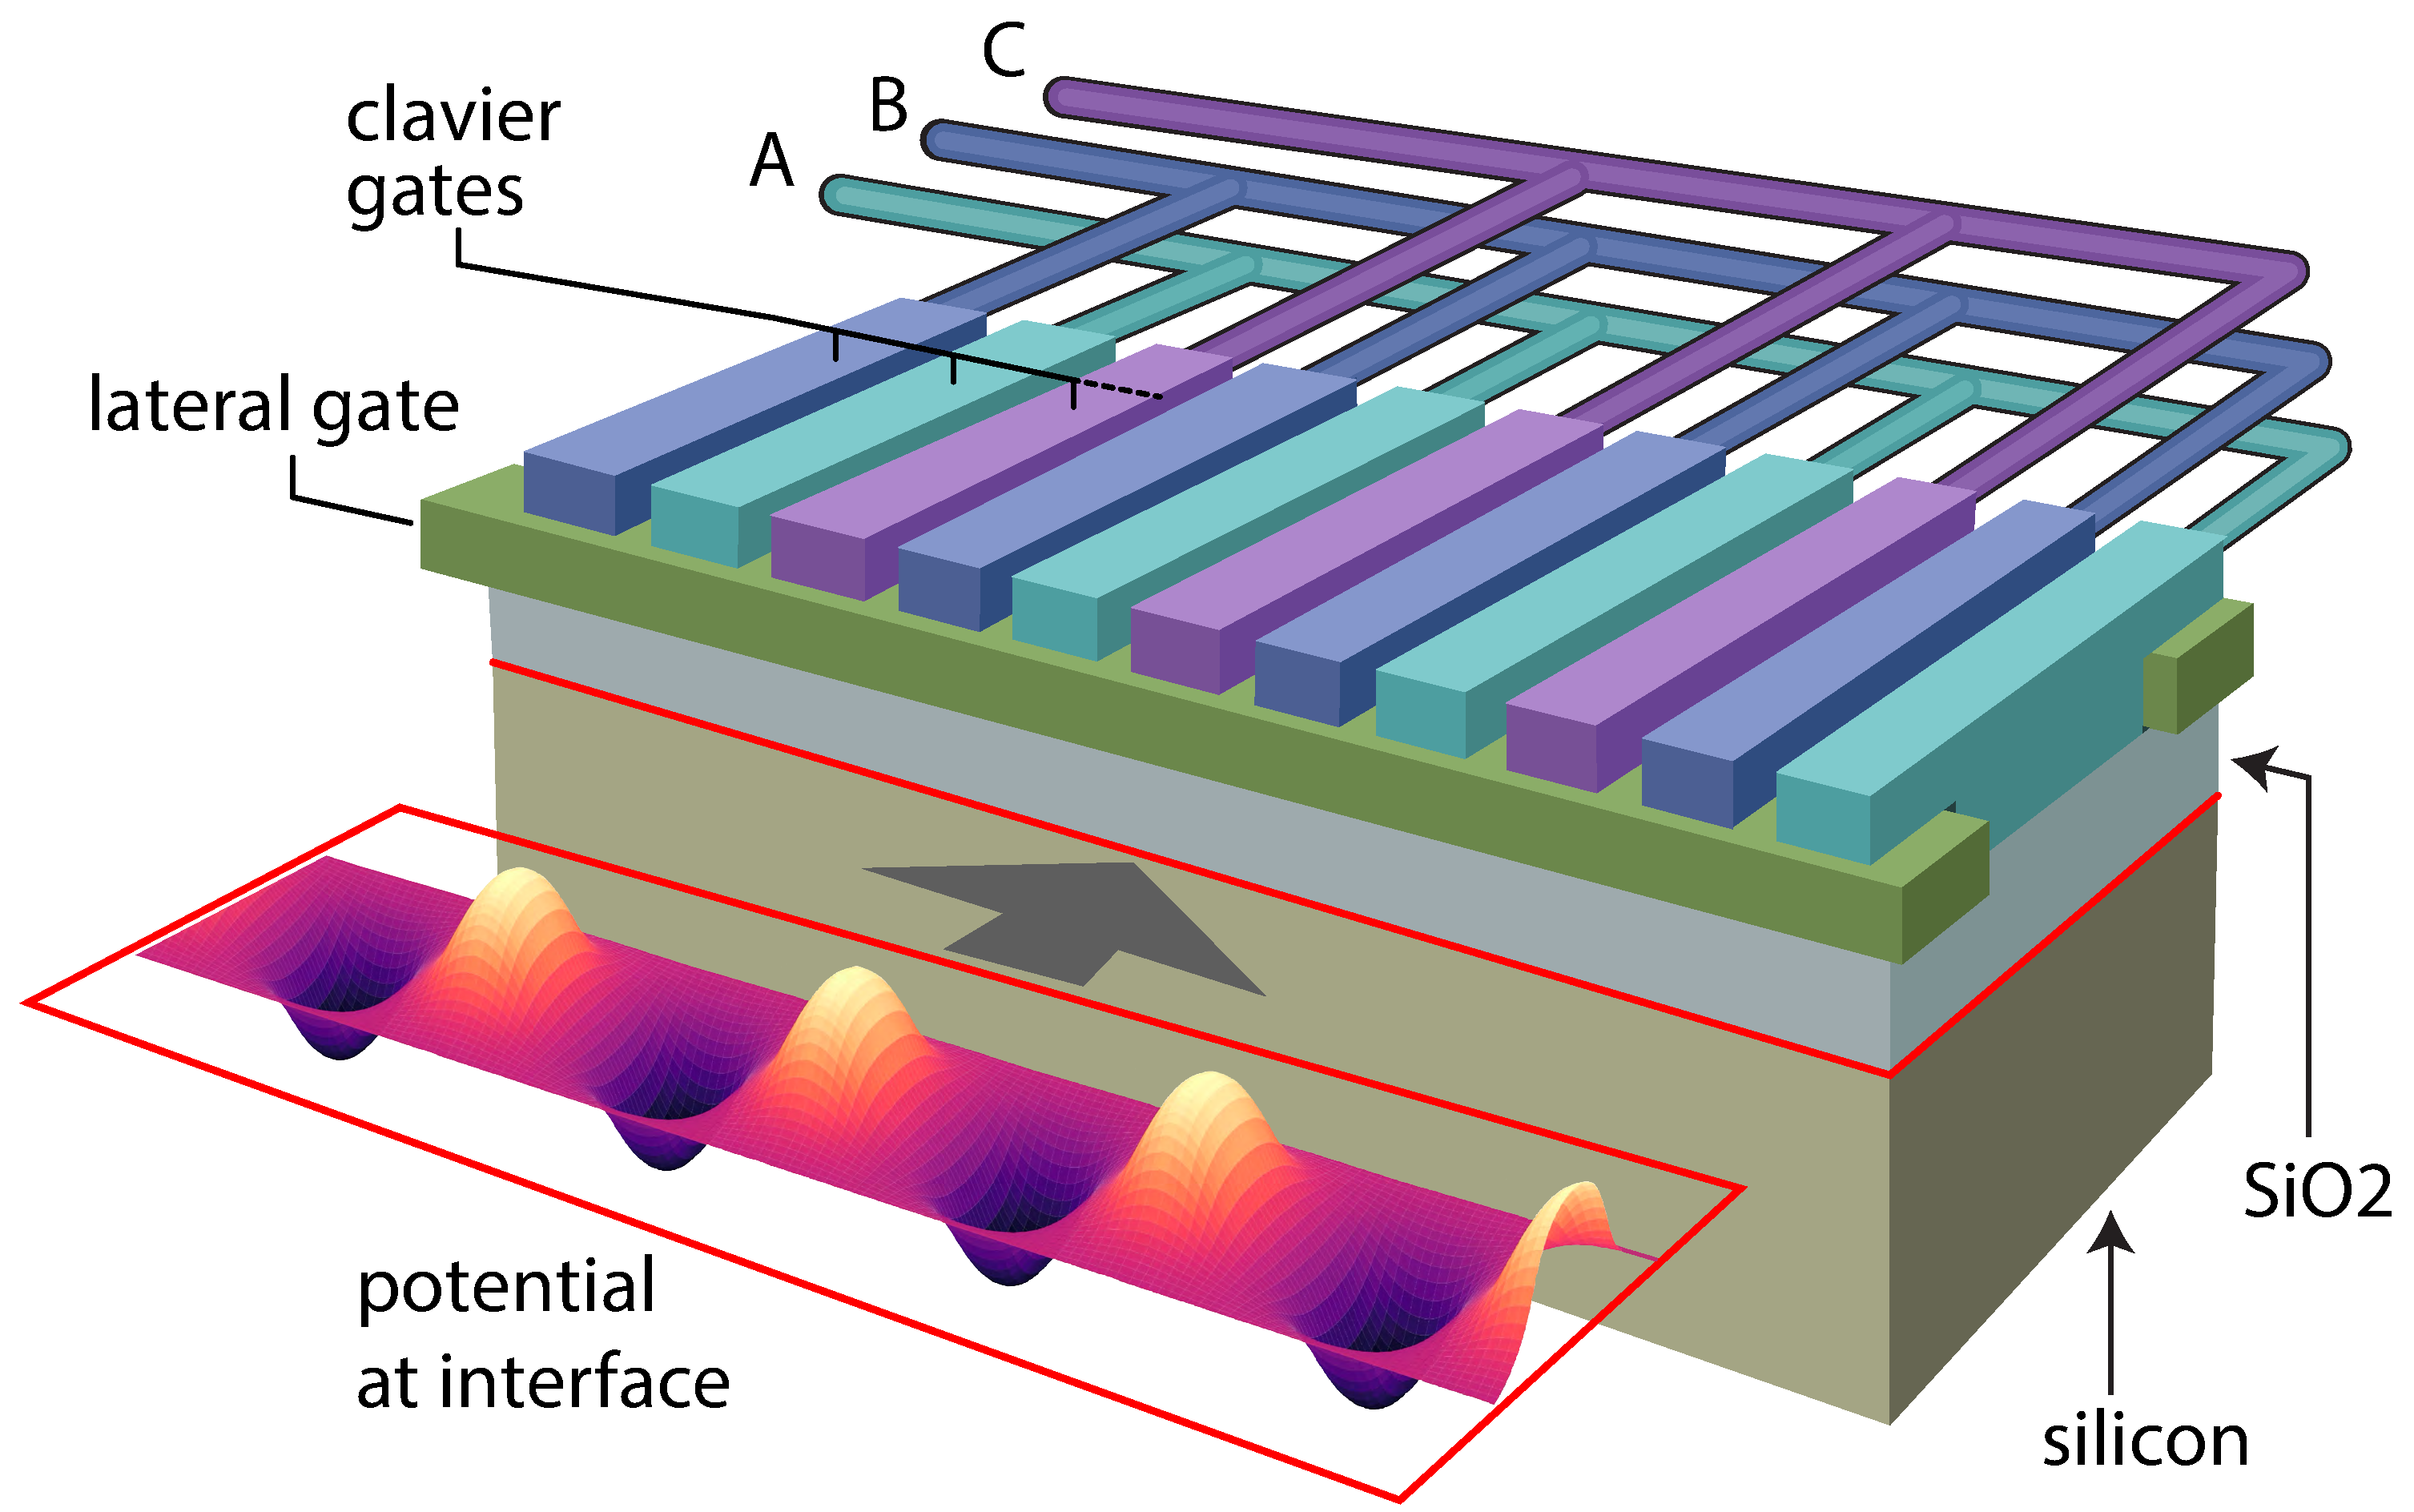
\includegraphics[width=\textwidth]{figures/ch2-shuttling/fancy3DfigSmV3.pdf}
    \caption{Conceptual illustration of the conveyor-belt shuttling device studied in this paper.  The electrons are confined near a silicon-oxide interface below a periodic array of gates to which external potentials can be applied via voltage lines A, B and C. In this paper we consider devices with three repeating electrodes, as depicted, as well as four\,\cite{langrock_2023} and five.}
    \label{fig:device_layout}
\end{figure}

\begin{figure}
\centering
\subfloat[]{%
	\includegraphics[width=\linewidth, trim={1cm 0.39cm 0 0.6cm},clip]{figures/ch2-shuttling/gate_geometry.pdf}\label{fig:device_geometry_3D}
}%

\hfill

\subfloat[]{%
	\includegraphics[width=\linewidth,trim={0.25cm 0 0 1.25cm}, clip]{figures/ch2-shuttling/gate_geometry_cross_section.pdf}\label{fig:device_geometry_cross_section}
}%

\caption{Illustration of (a) the shuttling device in 3D and (b) its cross-section in the xz plane. The yellow boxes are clavier gates with width and height of $30$\,nm along the x and z direction and the length of $75$\,nm along the y direction. The gap between the gates is $5$\,nm. The size of this unit cell with three gates is $105$\,nm along the shuttling direction, i.e the x-direction. The clavier gates are implanted in the oxide layer (blue). Below the oxide layer, there is a \ce{Si} layer (magenta), whose base is grounded.}
\label{fig:device_geometry}
\end{figure}

Shuttling of an electron is achieved by creating a moving QD using a set of voltage pulses applied to metallic gates. Here, we explore shuttling devices broadly consistent with the Spin Qubit Shuttle (SQS) proposed by Langrock et al.\cite{langrock_2023}. A significant distinction is that while Langrock et al. focused on a silicon/silion-germanium device, here we consider devices consistent with silicon/silicon-oxide structures. Figure~\ref{fig:device_layout} shows a sketch of the device; Figure~\ref{fig:device_geometry} indicates the key dimensions. At the top surface, a periodic array of so-called clavier gates is deposited in the shuttling direction. The clavier gates are embedded inside the \ce{SiO2} layer. The electron moves in a channel, which is located near the interface of \ce{Si} and \ce{SiO2}. To confine the electron to move only in one direction, two lateral confinement gates are deposited just below the clavier gates and a large negative voltage (typically around $-1$\,V) is applied to these. Finally, the bottom of the device is grounded, i.e. $0$\,V. The voltages on the clavier gates form a periodic array of quantum dots along the channel; a single electron is initially loaded from a single-electron transistor (SET) into the leftmost dot, then shuttled along the channel by varying the clavier gate voltages until it reaches a second SET at the right-hand end. 

We made a number of simplifications to model this device. First, we assumed that the confinement gates have a sufficiently strong negative voltage that they act like hard walls at the sides of the channel. Second, since the electron moves below the confinement gates, we assumed that the effective potential it experiences is formed only by those parts of the clavier gates that are not screened by the confinement gates. Third, we assume there are infinitely many clavier gates lined up in a row in the shuttling direction. Finally, we assume that the confinement in the z-direction is very strong, and the quantum dots are formed nearly at the interface of the \ce{Si} and \ce{SiO2}\cite{burkard_2023}.


Given these assumptions, our device model is illustrated (for the case of three independent electrode voltages) in Figure~\ref{fig:device_geometry}. The yellow boxes denote the clavier gates, the blue area denotes \ce{SiO2}, and the magenta box represents the \ce{Si}. Figure~\ref{fig:device_geometry_3D} shows a 3D illustration of the full device while Figure~\ref{fig:device_geometry_cross_section} shows a cross-section of the device through the centre of the channel. The dimensions of the clavier gates are $(h,w,l)=30$\,nm $\times 30$\,nm $\times 75$\,nm , while the gap between the electrodes is fixed to $5$\,nm. Furthermore, the interface between the \ce{Si} and \ce{SiO2} is $10$\,nm below the bottom of the clavier gates as shown in Figure~\ref{fig:device_geometry_cross_section}.

The Hamiltonian of the electron in 3D is given by 

\begin{equation}\label{eqn:time_dependent_hamiltonian_noise_free_3D}
    H = \frac{1}{2} \mathbf{p}^{T}M^{-1}\mathbf{p} - e\Phi(V_{0}(t), V_{2}(t), ..., V_{N-1}(t)),
\end{equation}where $M$ is the anisotropic mass tensor in silicon, and $N$ is the number of gates per unit cell. Note that the potential, $\Phi$, is a function of time-dependent gate voltages. 

In this paper, we ran simulations in 2D, using only the transverse electron mass, i.e. $m^{*} = 0.19m_{e}$ (See section \ref{sec:numerical_simulation} and appendix \ref{appendix:subsec:airy_function}). This reduces the Hamiltonian to

\begin{equation}\label{eqn:time_dependent_hamiltonian_noise_free_2D}
    H = \frac{1}{2m^{*}} \mathbf{p}^{2} - e\Phi_{Si/SiO_{2}}(V_{0}(t), V_{2}(t), ..., V_{N-1}(t)),
\end{equation} where we sample the 2D potential $\Phi_{Si/SiO_{2}}$ from the 3D potential, $\Phi$, at the \ce{Si}--\ce{SiO2} interface (See section \ref{sec:numerical_simulation}). Aside from our investigation of charge defects in section \ref{sec:charge_defects}, the form of Hamiltonian in equation \ref{eqn:time_dependent_hamiltonian_noise_free_2D} doesn't change; However, the time-dependent gate voltages change due to, e.g., the Johnson-Nyquist noise in section \ref{sec:johnson-nyquist} or different pulse shapes in section \ref{sec:snap}.

\section{Voltage profiles for conveyor-belt Shuttling}\label{sec:conveyor_belt_shuttling}
\begin{figure*}
	\begin{minipage}[t]{0.495\columnwidth}
  	\centering
        \subfloat[]{%
	\includegraphics[trim={0 4.0cm 0 0}, width=\linewidth]{figures/ch2-shuttling/repeating_voltage_signals.pdf}\label{fig:CB_mode_pulse_illustration_periodicity}}%
        
        
        \hfill
        
        \subfloat[]{%
	\includegraphics[trim={0 0.75cm 0 0},clip,width=\linewidth]{figures/ch2-shuttling/voltage_signals.pdf}
          \label{fig:CB_mode_pulse_illustration_sinusoidal}}%
    
        \hfill
    
        \subfloat[]{%
	\includegraphics[width=\linewidth]{figures/ch2-shuttling/potential_max_position_n_3.pdf}
          \label{fig:potential_max_x}}%
	\end{minipage}
	\hfill
    \begin{minipage}[t]{0.495\columnwidth}
        \subfloat[]{%
	\includegraphics[trim={0.70cm 0cm 0 0cm},clip, width=0.95\linewidth]{figures/ch2-shuttling/shuttling.pdf}
    \label{fig:CB_mode_pulse_illustration_shuttling}}%
        
        \hfill

        \subfloat[]{%
	\includegraphics[width=\linewidth]{figures/ch2-shuttling/potential_max_curvature_n_3.pdf}
          \label{fig:potential_max_curvature}}%
    \end{minipage}%
    
    \caption{Illustration of the voltage pulses applied to the gates in conveyor-belt shuttling for three gates per unit cell, i.e. $N=3$. (a) Every 3rd gate is connected to the same voltage source (denoted as red, green and blue lines). (b) The three independent pulses are sinusoidal with $2\pi/3$ phase difference. (c) The position, $x$, of the potential minimum as a function of time when the average shuttling speed is $10$\,m/s. The lines correspond to different choices of phase variation, $\phi(t)$: linearly varying phase $\phi(t)= k \cdot t$ (blue line), and phase obtained by using a look-up table, $f^{-1}$, $\phi(t)=f^{-1}(x(t))$ (orange line). The detailed arguments are given in Appendix~\ref{appendix:subsec:phase_variation}. (d) The resulting time-evolution of the potential and approximate position of the electron wave packet. The red, green, and blue boxes above denote the same clavier gates of the corresponding colour in (a) and (b). (e) Variation of the curvature at the potential minimum, $\kappa$, obtained by fitting the slice of potential energy at $y=0$ with a quadratic function (see also the plots of the full potential in Figure~\ref{fig:potential_3d_n_4}). Note that panels (a),(b), and (c) relate the panels (e), (f), and (g) of Figure 2 of  Langrock et al.\cite{langrock_2023}.}
    \label{fig:CB_mode_pulse_illustration}
\end{figure*}


\begin{figure*}
\subfloat[]{%
	\includegraphics[trim={1cm 1cm 1cm 1cm}, clip, width=0.495\textwidth]{figures/ch2-shuttling/3d_plot_potential_n_4.pdf}\label{fig:potential_3d_n_4_3d_1}
}%
~
\subfloat[]{%
	\includegraphics[width=0.495\textwidth]{figures/ch2-shuttling/contour_plot_potential_n_4_1.pdf}

  \label{fig:potential_3d_n_4_contour_1}
}%
\hfill
\subfloat[]{%
	\includegraphics[trim={1cm 1cm 1cm 1cm}, clip, width=0.495\textwidth]{figures/ch2-shuttling/3d_plot_potential_n_4_2.pdf}

  \label{fig:potential_3d_n_4_3d_2}
}%
~
\subfloat[]{%
	\includegraphics[width=0.495\textwidth]{figures/ch2-shuttling/contour_plot_potential_n_4_2.pdf}
  \label{fig:potential_3d_n_4_contour_2}
}%

\caption{3D and contour plots of the potential energy, $V(x,y)$, generated by the gates for $N=4$ with $A = 100$\,mV. (a) 3D  and (b) contour plots of the potential energy for one unit cell centred around the potential minimum when the curvature near the potential minimum, $\kappa(\phi)$, is maximum (corresponding to a potential well directly below an electrode). (c) 3D  and (d) contour plots of the potential energy for one unit cell centred around the potential minimum when $\kappa(\phi)$ is a minimum (corresponding to a potential well between two electrodes).}
\label{fig:potential_3d_n_4}
\end{figure*}


Conveyor-belt shuttling is achieved by creating a single QD moving in a desired trajectory (along the positive $x$ direction in our case). As explained in Langrock et al.\cite{langrock_2023}, such a potential can be created by applying sinusoidal voltage signals to the gates with a phase difference of $2\pi/N$ between successive gates; $N$ is then the number of independent voltage signals required:
\begin{equation}\label{eqn:sinusoidal_voltage_pulses}
    V_{i}(t) = A\cos(\phi(t) - \frac{2\pi i}{N}),
\end{equation}
where $A$ and $\phi(t)$ are the amplitude and phase of oscillation, respectively. Figure~\ref{fig:CB_mode_pulse_illustration_periodicity}  illustrates the repeating voltage signals; using an analogy from condensed-matter physics, we define a sequence of $N$ adjacent gates as a \textit{unit cell}. To be specific, the size of the unit cell along the shuttling direction, i.e. the x-direction, changes with the number of gate per unit cell, $N$. For example, the length of a unit cell is $105$\,nm for three gates per unit cell, but $175$\,nm for five electrodes per unit cell. Such a scheme solves the signal fan-out problem because the device only needs $N$ control lines regardless of the number of gates. For example, in the case of 4 gates in the unit cell, the applied pulses will be $\cos(\phi(t))$, $-\sin(\phi(t))$, $-\cos(\phi(t))$, and $\sin(\phi(t))$, where $\phi(t)$ is the phase as a function of time. The resulting evolution of voltage pulses at the clavier gates with time is illustrated in Figure~\ref{fig:CB_mode_pulse_illustration_sinusoidal}. To give a sense of direction, there must be at least three gates per unit cell.  Figure~\ref{fig:CB_mode_pulse_illustration_shuttling} shows the wave function propagating from left to right using the conveyor-belt shuttling at $4$ different times.

These voltage signals will successfully drive shuttling if the process proves to be adiabatic and thus the wave function closely follows the minimum of the potential energy. The instantaneous speed of shuttling is proportional to the first derivative of the phase $\phi(t)$ in the sinusoidal pulses. Hence, the shuttling trajectory depends on how the phase $\phi(t)$ is varied. We examined two possible ways to vary this phase: the first was a simple linear variation, while the second was designed to achieve a uniform propagation speed for the minimum of the quantum dot potential, the phases themselves being determined from a position-phase look-up table. Figure~\ref{fig:potential_max_x} shows the shuttling trajectories and voltage pulses (inset) for these two different methods of phase variation. 
However, a detailed comparison between the linearly increased phase and the phase obtained from the look-up table (in Appendix \ref{appendix:subsec:phase_variation}) showed that there is little practical difference between the two methods. Thus, we chose to update the phase linearly because it is easier to generate simple sinusoidal pulses on-chip than to apply more complicated pulses.

\section{\label{sec:numerical_simulation} Numerical Simulations}

For a given device geometry, specified as in section \ref{sec:shuttling_device}, it is necessary to solve the Laplace equation to obtain the QD potential, $\Phi(x,y,z,t)$, and then to solve the time-dependent Schr\"{o}dinger equation to simulate the dynamics of the shuttling. Periodic boundary condition was chosen along the shuttling direction, i.e. the x-direction, and $V=0$ was chosen for the bottom surface and sides of the shuttling track. In between the gates, Neumann boundary conditions of $\partial{\phi}/ \partial{z} = 0$ was imposed. At the \ce{Si}-\ce{SiO2} interface, the continuity of the displacement field was imposed, and the relevant relative permittivity for \ce{Si} ($11.69$) and \ce{SiO2} ($3.9$) were used. A detailed description of the boundary conditions is outlined in Appendix~\ref{appendix:subsec:boundary_conditions}. For the Poisson solver, we defined a uniform rectangular grid in 3D with finite difference approximation for the differential operators. We used successive over-relaxation (SOR)\cite{Young_1954, Frankel_1950} to obtain the time-dependent potential in the unit cell in Figure~\ref{fig:device_geometry}. For faster generation of the time-dependent potential, we used the superposition principle, based on the linearity of the Laplace equation, as noted in equation~\ref{eqn:superposition_principle_potential} in Appendix~\ref{appendix:subsec: numerical algorithms}. On the other hand, for the Schr\"{o}dinger solver, we used uniform rectangular grid in 2D on the plane defined by $z=-10$\,nm. We used the split operator method\cite{glowinski2017splitting} with symmetric Strang splitting\cite{strang1968construction, strang2012essays} to solve the time-dependent Schr\"{o}dinger equation. The convergence of the numerical methods were test in Appendix~\ref{appendix:subsec:convergence_studies}. Finally, the choices of unit systems and hyperparameters of the numerical methods are given in Appendix~\ref{appendix:subsec:Model}.

If we assume that the $z$-axis confinement is so strong that the electron only moves in the plane of the \ce{Si/SiO2} interface, modelling in 2D is enough to capture the relevant physics. The perpendicular extent of the wave-function is anyway reduced because the lowest-energy bound states are formed from the $\pm z$-valleys, so the motion in the $z$-direction is determined by the longitudinal (heavy) electron mass. Furthermore, \ce{SiO2} has large band gaps that allow strong electric fields to confine electrons in the z-direction without leakage out of the channel\cite{burkard_2023}. As a result, the typical confinement length of the QD in the $z$-direction is of order $1$\,nm\cite{Yang2013-wr, Veldhorst_2015, Ruskov_2018} while the oxide layer thickness is $10$\,nm. Thus, we sampled our 2D potential at the interface between \ce{Si} and \ce{SiO2}. A detailed comparison of the potential sampled at the interface and the potential averaged over the probability density of the ground state in the z-direction is given in Appendix~\ref{appendix:subsec:airy_function}.

We may further reduce the dimensionality to 1D if we assume that the voltages at the confinement gates are so high that the electron never undergoes excitation in the $y$-direction. A detailed comparison of 1D and 2D simulations is given in Appendix~\ref{appendix:subsec:1d_vs_2d}. 1D and 2D simulations yield different loss probabilities and excitation fractions with an order of magnitude difference for realistic parameters. This highlights the importance of simulating in 2D and that the potential is non-separable. We therefore report results of the more accurate 2D simulations in the remainder of the paper.

Note that the atomic scale interface roughness was neglected in our simulations.  Given that interface roughness has a similar nature to the Johnson-Nyquist noise, the results of section \ref{sec:johnson-nyquist} imply that it only affects the orbital excitation if there is a frequency component in the moving frame of the electron that is comparable to the energy gap in the orbital degree of freedom. For example, if the shuttling speed is $100$\,m/s and the smallest length scale of roughness is, say, $0.5$\,nm, the maximum change in frequency is $0.2$\,THz, which is much smaller than the frequency of characteristic energy gap, i.e. $\Delta E_{gs,2e}/h = 1.46$\,THz. 

We also neglect the effect of valley physics.  This is likely to have minimal effect on charge shuttling: valley-orbital anti-crossings are unlikely to occur because the four transverse valley states have much higher energy than the $\pm z$-valleys. In any device where the tensile strain in \ce{Si} exceeds $0.1$\,\%, the transverse valley states lie more than $20$\,meV above the $\pm z$-valleys~\cite{Euaruksakul_2008}, comfortably higher than our characteristic orbital energy gap of $6.02$\,meV ($A=100$\,meV and $N=4$ electrodes per unit cell). Furthermore, given strong confinement in the z-direction (confinement length $\sim 1$\,nm), there is an additional contribution to the splitting from the effective mass anisotropy (the longitudinal mass is around $5$ times bigger than the transverse mass).  On the other hand, the lowest valley excitation occurs within the $\pm z$-valleys and lies well below the orbital excitations (The energy scale of excited valley states is $\mathcal{O}$($10$-$100$\,$\mu$eV) while the energy scale of orbital states is  $\mathcal{O}$($1$\,meV)); it is not resolved in our calculations but does not significantly affect the location of the shuttled charge.  Therefore, valley-orbital anti-crossings are unlikely unless the tensile strain is unusually small. 

\section{\label{sec: metrics} Performance metrics}

\begin{figure}
    \centering
    \includegraphics[width=\columnwidth]{figures/ch2-shuttling/loss_prob_explanation.pdf}
    \caption{Illustration of the definition of the loss probability as the integrated probability density (orange line) over the shaded region  $\nu$, defined as the region outside the well in potential energy (blue line) being used to shuttle the electron.}
    \label{fig:loss_prob_metric}
\end{figure}

We will characterise the shuttling process by evaluating its capability to move the spin qubit to the target position (1) without losing the qubit and (2) with a good degree of adiabaticity. Specifically, the excitation in the orbital state is important as the $g$-factor of the electron in silicon depends both on its position and orbital state\cite{Kawakami_2014, langrock_2023}. Thus, the two most import imperfections to evaluate the shuttling scenarios are (1) the probability $P_L$ of losing the electron from the potential well and (2) the amount of excitation from the ground state. 

The loss probability is defined as the probability that the electron is found outside the single QD where it was initially loaded. Since we have periodic boundary conditions along the x-axis, we need at least two unit cells, i.e. two QDs, to calculate the loss probability. When there are two unit cells, the loss probability is equivalent to the probability of the electron to be in the other `wrong' QD (since we solve the TDSE only within the channel region, the electron cannot leave the channel). Figure~\ref{fig:loss_prob_metric} shows the illustration of calculation of loss probability. The loss probability is the probability in the shaded region, $\nu$:
\begin{equation}
    P_{L} = \int\limits_{\nu} dxdy \, |\psi(x,y)|^2 
\end{equation}where $\psi(x,y)$ is a 2-dimensional wave function.

The excitation fraction is a dimensionless measure of the level of excitation of the system due to non-adiabatic effects. It is defined as the ratio $\Delta E/\Delta E_{gs,2e}$ where $\Delta E$ is difference between the expectation value of the energy and the (instantaneous) ground state energy and $\Delta E_{gs,2e}$ is a characteristic energy gap; it should be interpreted as the excess energy relative to this characteristic energy gap. Since the excitation primarily occurs in the direction of shuttling, the characteristic energy gap was chosen as the energy gap of the ground to the second excited state, so that $\Delta E/\Delta E_{gs,2e} =  (E - E_{gs})/(E_{2e} - E_{gs})$. Figures~\ref{fig:fidelity_gamma} and  \ref{fig:fidelity_temperature} show that excitation primarily populates the second excited state, which is the excitation mode in the x-direction as shown in Figure~\ref{fig:excited_states_2d}.

Additionally, we calculated the probabilities of excitation to the $n$th eigenstate of the instantaneous Hamiltonian. This metric was used to compare the performance of the noisy shuttling cases, as the fidelity between the final state and the ground state deviates from $1$ by the order of only $10^{-7}$ for noise-free shuttling.

When we report metrics for the overall performance of the shuttling experiment, these are computed using the state of the system during the static phase after the shuttling procedure. The static phase involved an additional 5000 times steps ($\approx 13.5$\,ps) to evolve the state with the stationary potential at the end of the shuttling. While the excitation fraction remains constant up to a numerical precision during this period, the loss probability may vary if the potential barrier is too low, much lower than our default setting of $100$\,mV. Effectively, we sampled one loss probability value in this case; These scenarios, however, correspond to a failed shuttling, and any small fluctuation in loss probability is not of much interest.

\section{\label{sec: noiseless_shuttling}Noiseless Shuttling}
\begin{figure*}
	\subfloat[]{% 
	\includegraphics[width=0.495\textwidth]{figures/ch2-shuttling/loss_V_max_n_all_table_0_log.pdf}
    \label{fig:loss_probability_amplitude}}
    ~    
    \subfloat[]{%
    \includegraphics[width=0.495\textwidth]{figures/ch2-shuttling/excitation_fraction_V_max_n_all_table_0_log.pdf}
	
    \label{fig:loss_probability_target_dist}}%

    \hfill	
    \subfloat[]{% 
	\includegraphics[width=0.495\textwidth]{figures/ch2-shuttling/loss_target_dist_n_all_table_0_log.pdf}
    \label{fig:excitation_fraction_amplitude}}%
    ~    
    \subfloat[]{\includegraphics[width=0.495\textwidth]{figures/ch2-shuttling/excitation_fraction_target_dist_n_all_table_0.pdf
    }
    \label{fig:excitation_fraction_target_dist}}%

    \caption{The loss probability and excitation fraction for different noiseless shuttling scenarios: (a) loss probability and (b) excitation fraction as a function of voltage signal amplitude, $A$, for a shuttling distance of $1.4$\,$\mu$m; (c) loss probability and (d) excitation fraction as a function of target distance, $D$, for a signal amplitude of $100$\,mV.  Results for different numbers of electrodes per unit cell ($N=3,4,5$) are shown.}
    \label{fig:loss_and_excitation_target_dist}
\end{figure*}

In this section, we present the results from shuttling scenarios where there is no noise and no defect charges are present. While the quality of shuttling depends on many parameters, we selected three independent variables: (1) the target distance, (2) the amplitude of the voltage signals at the gates, and (3) the number of gates in a unit cell. 

Figures~\ref{fig:loss_probability_amplitude} and \ref{fig:excitation_fraction_amplitude} show the loss probability and excitation fractions for different amplitudes of sinusoidal oscillations at the gates. Larger signal amplitudes make a deeper QD, and thus the loss probability decreases. Our typical value of amplitude, $100$\,mV, resulted in a loss probability of $3 \times 10^{-11}$ even for $N=3$ electrodes. The loss probability reduces even further for larger numbers of electrodes as the depth of the QD and the inter-dot distance both increase. For example, when the amplitude is $50$\,mV, we see a loss probability of $10^{-5}$ for $N=3$ while we see the similar loss probabilities for $N=4$ and $N=5$ when the amplitudes are $25$\,mV and $12.5$\,mV.

Figures~\ref{fig:loss_probability_target_dist} and \ref{fig:excitation_fraction_target_dist} show the loss probability and excitation fraction with different target distances. The mean shuttling speed and the amplitude of voltage signals were fixed to $10$\,m/s and $100$\,mV, respectively. As the target distance increases, both the loss probability and excitation fraction increase. The worst case occurs when the number of electrodes is three and the target distance is $8.4$\,$\mu$m, which nevertheless results in near-ideal behaviour:  a loss probability of $1.3 \times 10^{-10}$ and an excitation fraction  of $2.7 \times 10^{-7}$.

Given these data, we conclude that noiseless shuttling is practically perfect when the default speed and amplitude were used with the target distance up to $8.4$\,$\mu$m. The quality of shuttling significantly depends on the amplitude of the voltage signal and the number of gates per unit cell. To reduce the loss probability, it is always beneficial to use more gates per unit cell; but for a broad range of cases we find that $N=3$ is quite sufficient for near-ideal performance.

\section{Sensitivity to Johnson-Nyquist noise} \label{sec:johnson-nyquist}

Since noise-free shuttling is nearly perfect, we further investigated the effect of discontinuities in the voltage signals. The full results are described in Appendix~\ref{appendix:subsec:step_changes} and we summarise here. Two extreme cases were studied: staircase-like potentials in time, with step-changes in the potential at defined intervals, and potentials formed from piece-wise linear functions connecting the midpoints of the steps of the staircase-like potential (See Figure~\ref{fig:voltage_signals_mode1_vs_mode2}). From Figure~\ref{fig:loss_and_excitation_step_vs_linear}, we concluded that staircase-like discontinuities in the voltage signals result in much more loss and excitation than continuous signals. 

Fortunately, these staircase-like voltage profiles  constitute an adversarial model that is somewhat unphysical, as in reality there is a finite response time for any change of voltage at the gates. However, rapid changes in the gate voltages on frequencies up to this cutoff can still arise from Johnson-Nyquist noise \cite{Johnson1927-ag, Nyquist_1928}, which is a thermal noise at the resistor caused by random thermal agitation. We therefore proceed to explore the impact of such noise when physically motivated. 

Figure~\ref{fig:circuit} shows a lumped-element model of a voltage source connected to clavier gates via a single bondwire. $L$ is the inductance of the bondwire, $R$ is the resistance of the metal connection from the bondpad to the gate, $C_{1}$ is the capacitance of the bondpad, and $C_{2}$ is the capacitance of clavier gate. (See appendix \ref{appendix:subsec:lumped_element_model}) The power spectral density of classical Johnson-Nyquist noise can be derived as
\begin{equation} \label{eqn:PSD_johnson_nyquist_classical}
    S_{C}(\omega) = 4k_{B}T \frac{N_{G}C_{2}}{C_{1}^2} \frac{\gamma}{\omega^{2} + \gamma^{2}},
\end{equation}where $\gamma=\frac{1}{RC_{2}}$ is the characteristic inverse time constant of the Lorentzian distribution and $N_{G}$ is the number of gates and metal connections connected to the same bondpad, as shown in the left side of Figure~\ref{fig:circuit}. The corresponding RMS voltage noise can be obtained as
\begin{equation}\label{eqn:rms_noise_temperature} 
    \Delta V_{\text{rms}} = \sqrt{2\pi k_{B}T \frac{N_{G}C_{2}}{C_{1}^{2}}}.
\end{equation}

\begin{figure}

\subfloat[]{%
	\includegraphics[width=\linewidth]{figures/ch2-shuttling/PSD_no_zero_point_term.pdf}
  	\label{fig:PSD_Johnson_Nyquist}
}%

\hfill

\subfloat[]{%
	\includegraphics[width=\linewidth]{figures/ch2-shuttling/quantum_classical_noise_no_zero_point_term.pdf}
  	\label{fig:quantum_classical_noise_comparison}
}%

\caption{(a) the power spectral density, $S$, of the classical (blue) and quantum (orange) Johnson-Nyquist noise, and (b) random instances of classical (blue) and quantum (orange) Johnson-Nyquist noise, $V_{noise}$, at $T=4$\,K, and $\gamma=10$\,THz}
\label{fig:eta_PSD_johnson-nyquist_noise}
\end{figure}

We first looked into the effect of classical Johnson-Nyquist noise. The complete results are described in Appendix~\ref{appendix:subsec:johnson-nyquist_classical}, and we summarise here. Figure~\ref{fig:loss_and_excitation_gamma_temp_classical} shows that both loss probability and excitation fraction significantly increase with higher cut-off frequency, $\gamma$, and higher temperature, $T$. We concluded that high frequency noise, especially the one that is comparable to the frequency corresponding to the characteristic energy gap, i.e. $\Delta E_{gs,2e/\hbar}$, is more harmful than low frequency noise. For example, for our default setting of $4$ gates per unit cell and the amplitude of the voltage signal of $100$\,mV, i.e. $N=4$ and $A=100$\,mV, the resulting characteristic energy gap is around $6$\,meV, which corresponds to the frequency of $1.46$\,THz, i.e. $\Delta E_{gs,2e}/h = 1.46$\,THz.

In reality, quantum effects have to be taken into account once the cut-off frequency reaches $\gamma \gtrsim k_BT/\hbar$. To account for this\,\footnote{There has been a debate about whether to include the zero-point fluctuations in the correction term\cite{Kish_2016}, which is an additive term of $\hbar\omega/2k_{B}T$ to the correction factor. We found that our situation is close to an example by Kish et al.\cite{Kish_2016}, a resistor connected to an antenna with a photon counter. This is because the amount of fluctuation in the voltage of the gates is \textit{measured} by the electron shuttled underneath the gates, which acts like a photon counter in the example. Furthermore, note that spontaneous absorption doesn't exist while spontaneous emission exists due to the zero-point energy. Since the electron is absorbing energy from the gates, zero-point energy cannot be transferred to the electron, and this implies the absence of the zero-point term in the correction factor. A more detailed discussion about the inclusion of the zero-point term can be found in Kish et al.\cite{Kish_2016}.}, we multiply the Lorentzian power spectral density in equation \ref{eqn:PSD_johnson_nyquist_classical} by a correction factor $\eta(\omega)$ corresponding to the ratio between the thermal mode populations in the classical and quantum cases:
\begin{equation}
    \eta(\omega) =\frac{\hbar \omega/k_{B}T}{e^{\hbar \omega/k_{B}T} -1},
\end{equation}
\begin{equation} \label{eqn:PSD_johnson_nyquist_quantum}
    S_{Q}(\omega) = S_{C}(\omega)\eta(\omega).
\end{equation}
The correction factor decreases from $\eta(0) = 1$ as the frequency increases, with an asymptotic value of $\eta(\omega) = 0$. Since $\eta(\omega) \leq 1$ for all frequencies, the power spectral density now deviates from the pure Lorentzian distribution with the higher frequency components more strongly suppressed. Figure~\ref{fig:PSD_Johnson_Nyquist} shows the classical and quantum power spectral density at a temperature of $4$\,K and cut-off frequency $10$\,THz. For a given cut-off frequency $\gamma$, we expect that the quality of shuttling will be improved relative to the corresponding classical case owing to the smaller PSD at higher frequencies. Figure~\ref{fig:quantum_classical_noise_comparison} shows instances of classical and quantum noise generated with the same circuit elements at $T=4$\,K; the reduction in high-frequency noise in the quantum case is evident, and the total noise power decreases to only $5.5$\,\%  of the classical value.

Simulations of the noisy shuttling process were performed by generating random noise profiles from the power spectral density, by the procedure given in Appendix~\ref{appendix:subsec:generation_of_noise}. The values of the circuit elements in Figure \ref{fig:circuit} are given in appendix \ref{appendix:subsec:lumped_element_model}. The shuttling distance was chosen to be $1.4$\,$\mu$m, which corresponds to $10$ unit cells; thus, we assumed $10$ gates are connected via a single bondpad to a single voltage source with the total capacitance of $N_{G} \times C_{2} = 1$\,fF.

\begin{figure*}
\centering
    	\subfloat[]{%
    	 \centering
    \includegraphics[width=0.495\textwidth]{figures/ch2-shuttling/loss_quantum_noise_temperature_gamma.pdf}

          \label{fig:loss_quantum_noise_temperature}
    	}%
    	~
    	\subfloat[]{%
        \includegraphics[width=0.495\textwidth]{figures/ch2-shuttling/excitation_fraction_quantum_noise_temperature_gamma_log.pdf}
			
    \label{fig:excitation_fraction_quantum_noise_temperature}    	
    	}%
    \hfill
    \subfloat[]{%
        \centering
    \includegraphics[width=0.495\textwidth]{figures/ch2-shuttling/loss_quantum_noise_gamma_log.pdf}
          \label{fig:loss_quantum_noise_gamma}
    }%
    ~
    \subfloat[]{%
    \centering
    \includegraphics[width=0.495\textwidth]{figures/ch2-shuttling/excitation_fraction_quantum_noise_gamma_log.pdf}
    \label{fig:excitation_fraction_quantum_noise_gamma}
    }%
    
    \label{fig:loss_excitation_fraction_qauntum_noise}
    \caption{Loss probability and excitation fraction: (a, b) as a function of temperature with three different cut-off frequencies, i.e. $\gamma=10, 100, 1000 GHz$ for three gates per unit cell ($N=3$) and (c, d) as a function of cut-off frequency $\gamma$ with varying number of gates per unit cell, $N$.}
    
\end{figure*}

Figures~\ref{fig:loss_quantum_noise_temperature} and \ref{fig:excitation_fraction_quantum_noise_temperature} show the loss probability and excitation fraction for three gates per unit cell, i.e. $N=3$, at different temperatures $T$ ranging from $0.1$\,K to $10$\,K and with varying cut-off frequencies, $\gamma = 10,\ 100,\ 1000$\,GHz. For all cut-off frequencies, the excitation fraction tends to increase with temperature. However, there is highly significant increase only for $\gamma=1000$, where loss is seen to increase by three orders of magnitude (with an appreciable climb starting at lower temperatures). The excitation fraction also increases with both temperature and $\gamma$.

However, while both loss and excitation are finite and can rise severely with temperature, the primary conclusion is that they remain practically negligible. If we make the assumption that shuttling of qubits will not occur above a $4$\,K, we can confirm that at this temperature there is near-ideal behaviour. One observes that $P_L$ is always below $10^{-10}$ and the excitation fraction remains below $10^{-3}$ for all three architectural variants $N=3,\,4,\,5$.

\begin{figure}
    \centering
    \includegraphics[width=\textwidth]{figures/ch2-shuttling/exc_frac_p_gs_vs_time_N_3_10.pdf}
    \caption{Probability of excitation outside of the ground state (blue) and excitation fraction during the shuttling (orange) for a target distance of $1.4$\,$\mu$m at $10$\,m/s. Other parameters were set as follows: The amplitude of voltage signals was $50$\,mV, i.e. $A=50$\,mV, the temperature was $2$\,K, i.e. $T=2$\,K, and there were three gates per unit cell, i.e. $N=3$.}
    \label{fig:infidelity_exc_frac_along_distance}
\end{figure}

Additionally, to confirm that there is no excitation during the shuttling process, we noted down the probability to remain in the ground state and excitation fraction in the middle of shuttling. Figure~\ref{fig:infidelity_exc_frac_along_distance} shows the probability of excitation outside of the ground state throughout the shuttling for a target distance of $1.4$\,$\mu$m at $10$\,m/s. During the shuttling, the probability of excitation was in the order of $10^{-6}$ to $10^{-5}$, the excitation fraction was in the order of $10^{-7}$ to $10^{-6}$ suggesting that the entire process of shuttling is largely adiabatic.

We conclude that, when high frequency components are suppressed by the correction factor, the effect of Johnson-Nyquist noise is negligible and the loss probability is comparable to the noiseless shuttling in the temperature ranges of practical interest. Furthermore, the entire process of shuttling remains adiabatic.

\section{Sensitivity to Charge Defects} \label{sec:charge_defects}

As Langrock et al.\cite{langrock_2023} pointed out, trapped charges due to impurities can affect the performance of shuttling if they occur near the interface defining the qubit layer. In this section, we investigate the effect of negative charge defects on the loss probability and excitation fraction. We used three unit cells and five electrodes per unit cell for these simulations, and the electron was shuttled across two unit cells in the presence of charge defects. Note that the trapped charges were placed in the oxide layer, and we used the permittivity of the oxide layer to compute the Coulomb peaks formed by the trapped charges. Since the oxide thickness is $10$\,nm (see section \ref{sec:shuttling_device}.), we chose the mid-point, i.e. $5$\,nm, as a default distance of defects from the interface. The Coulomb repulsion terms from the negatively charged defects are added to the Hamiltonian in equation \ref{eqn:time_dependent_hamiltonian_noise_free_2D}:

\begin{align}
    H &= \frac{\hbar^{2}}{2 m^{*}} \mathbf{p}^{2} - e\Phi(V_{0}(t), V_{2}(t), ..., V_{N-1}(t)) \\ \nonumber
    &+ \sum^{N_\text{\it defects}}_{i=1} \frac{e^{2}}{4\pi\epsilon_{0}\epsilon_{Si}|\mathbf{r} - \mathbf{r}_{i}|},
\end{align}where $\{r_{i}\}_{i = 1...N_\text{\it defects}}$ are positions of the charge defects in 3D space. Note that the motion of electron is still confined in a 2D space; The Coulomb repulsion from the static charges is calculated as if they are above (or below) the plane of motion in the 3D space. 

\begin{figure}
    \centering
    \includegraphics[width=0.9\textwidth,trim={0.40cm 0cm 0 0cm},clip]{figures/ch2-shuttling/loss_prob_no_window_height_5nm.pdf}
    \caption{The loss probability of electron wave function with varying number of charge defects, $N_{defects}$, in the channel. Note that, for each number of charge defects, $100$ random configurations of charges were simulated. Up to $N_\text{\it defects}=4$, the loss probability remains nearly zero while we start to see cases with high loss probability with more than 6 defects present. The blue line connects the mean loss probability for each $N_\text{\it defects}$.}
    \label{fig:loss_prob_varying_number_defects}
\end{figure}

Figure~\ref{fig:loss_prob_varying_number_defects} shows the electron loss probability in the presence of varying number of charge defects. We considered a range of $N_\text{\it defects}$, the total number of charge defects, and for each case we simulated $100$ random configurations. For $4$ or fewer charge defects, the loss probability remains near to zero; but this probability climbs for higher defect counts. Notably, for as few as 6 defects, we did observe at least one case where the loss probability exceeds 50\% -- a catastrophic failure of the shuttling channel where the electron is likely to be ejected from the confinement region. 

To investigate further we explored `adversarial' scenarios where we seek the worst-case positioning for a small number of defect charge(s). We initially simulate scenarios with a single trapped negative electronic charge in the centre of the channel located either $2$\,nm or $5$\,nm away from the interface, with varying shuttling speeds. We also simulated cases where two and three trapped charges are aligned at a given x-coordinate, and so are liable to form a potential wall to repel the shuttled electron. In particular, two and three charges were positioned symmetrically around the centre axis of the channel, i.e. $y=0$, with the distance between two adjacent charges to be $1/3$ and $1/4$ of the full width of the channel ($100$\,nm), respectively.

Contour plots of the potential energies with one, two, and three charges placed at $5$\,nm above the interface are shown in Figure~\ref{fig:countour_plots_charge_defects} at a time where the phases of the gate voltages alone would produce a minimum in the potential energy at the charge location.

\begin{figure}
	\subfloat[]{%
	\includegraphics[width=\linewidth]{figures/ch2-shuttling/contour_with_num_charge_1_num_unit_cells_3.pdf}
        \label{fig:contour_plot_one_charge_defect}
}%
    \hfill
    \subfloat[]{%
    \includegraphics[width=\linewidth]{figures/ch2-shuttling/contour_with_num_charge_2_num_unit_cells_3.pdf}
        \label{fig:contour_plot_two_charge_defect}
    }%
    \hfill
    \subfloat[]{%
    \includegraphics[width=\linewidth]{figures/ch2-shuttling/contour_with_num_charge_3_num_unit_cells_3.pdf}
        \label{fig:contour_plot_three_charge_defect}
    }%
    \caption{Contour plots of the potential energies with varying number of charge defects: (a) one, (b) two, and (c) three. Note that, for (b) and (c), the charges were aligned in the middle of the channel to form a wall to repel the electron. The distance from the interface to the charge defects was set to $5$\,nm.}
    \label{fig:countour_plots_charge_defects}
\end{figure}

Figure~\ref{fig:prob_gs_charge_defects} shows the probability of remaining in the ground state of the potential that would be formed by the gates alone (i.e., excluding the Coulomb potentials of the charge defects) when the shuttling speed is $10$\,m/s, and the shuttling distance is $350$\,nm (i.e., the length of two unit cells for $5$ electrodes). This means the electron was shuttled from one trough to the next, i.e. from one dark oval to the next in Figure~\ref{fig:countour_plots_charge_defects}. Thus, the electron is closest to the charge defects in the middle of the shuttling at around $17.5$\,ns. While the transfer is still almost adiabatic for one and two charge defects, for three defects the probability to remain in the instantaneous ground state of the gate potential drops to almost zero.  When the shuttled electron encounters the potential wall formed by the three charge defects, its wave functions becomes almost completely delocalized; it becomes unbound from its well in the shuttling potential. This is therefore a catastrophic failure of the shuttling process, and the device could not be used as a shuttling channel until/less the defect charges are moved.

It is unsurprising (indeed inevitable) that a sufficiently adversarial scenario involving multiple trapped charges will prevent shuttling. What is more remarkable is the protocol's robustness to the cases that might, intuitively, seem very problematic -- i.e. that it takes three trapped charges to `block' the channel with high probability. Figure~\ref{fig:prob_gs_charge_defects} shows that a single trapped charge or a pair of charges will imply a radical change to the instantaneous ground state, but the process can remain near-ideal. The contrast to the case of the three-charge `wall' is dramatic. 

We explored the worst case for the two-defect scenario. Figure~\ref{fig:two_charge_defects_varying_distances} shows the loss probability and excitation of the electron for varying defect separation, i.e. $\Delta y$. Both loss measures are at their most severe at about $\Delta y=25$\,nm. However, even at this point the loss is only $\approx4\%$; for separations outside a narrow $22$ to $27$nm range, the loss is again negligible. Figure~\ref{fig:potential_cross_section_defects_varying_dist} shows the cross-section of the potential on the $x=0$\,nm plane of figure \ref{fig:contour_plot_two_charge_defect} with varying defect separations. When the separation is small, e.g. $\Delta y=2$\,nm, the potential energy near the channel sides, e.g. $y \approx \pm 20$\,nm is low enough for the electron to move around the central barrier as in Figure~\ref{fig:two_charge_defects_varying_distances_states_2nm} in appendix~\ref{appendix:subsec:defects_varying_dist}. When the separation is large, e.g. $\Delta y = 30$\,nm, the potential energy in the middle is low enough for the electron to pass between the repulsive peaks as in Figure~\ref{fig:two_charge_defects_varying_distances_states_30nm} in appendix~\ref{appendix:subsec:defects_varying_dist}. However, at $\Delta y=25$\,nm, neither of these actions is easy: the local minima of potential energy($y=0,\pm ~ 25$\,nm) have roughly the same values as the potential energy at the channel edges ($y=\pm50$\,nm), and the electron requires higher energy to tunnel the barrier. Thus, Figure~\ref{fig:two_charge_defects_varying_distances_states_25nm} in appendix~\ref{appendix:subsec:defects_varying_dist} shows the high energy state of the electron tunneling through the barrier.

\begin{figure}[!ht]
	\subfloat[]{%
		\includegraphics[width=\linewidth]{figures/ch2-shuttling/prob_gs_123.pdf}
        \label{fig:prob_gs_charge_defects}
	}%
    \hfill
    \subfloat[]{%
		\includegraphics[width=\linewidth]{figures/ch2-shuttling/exc_frac_p_gs_vs_distance_charge_defects.pdf}
        \label{fig:two_charge_defects_varying_distances}
	}%
    \caption{(a) The probability to remain in the instantaneous ground state of the potential formed by the gates alone for a shuttling speed of $10$\,m/s and varying numbers of charge defects, $N_{defects}$: one (blue), two (orange), and three (green). The electron is closest to the defects in the middle of the shuttling. Note that, for one and two charge defects, the probability decreases temporarily below $0.2$ as the electron passes the defects but rises back to approximately $1$; for three charge defects, shuttling fails as the probability decreases to almost zero at the end of shuttling.The distance from the interface to the charge defects was set to $5$\,nm. (b) The loss probability and excitation fraction of the electron wave function in the presence of two charge defects, separated by $\Delta y$, for a shuttling speed of $10$\,m/s. $\Delta y = 0$ corresponds to two charges at the same location, equivalent to one charge defect with twice the charge. As $\Delta y$ increases the peak loss probability and excitation fraction are about $0.04$ and 4 respectively. }
    \label{fig:prob_gs_123_and_two_charge_defects_varying_distances}
\end{figure}

\begin{figure}
    \centering
    \includegraphics[width=\textwidth]{figures/ch2-shuttling/potential_y_cross_sections_two_defects.pdf}
    \caption{The cross-section of the potential in the $xz$ plane (at $x=0$\,nm in Figur~\ref{fig:contour_plot_two_charge_defect}) in the presence of two charge defects of varying separations $\Delta y= 2, 12 , 25, 30$\,nm. Each defect has charge of $-e$.}\label{fig:potential_cross_section_defects_varying_dist}
\end{figure}

Our simulations also confirm that charge defects closer to the shuttling channel are more harmful to shuttling at varying shuttling speeds (see Figure~\ref{fig:excitation_fraction_charge_defects}).

\begin{figure}
    \centering
    \includegraphics[width=\textwidth]{figures/ch2-shuttling/excitation_fraction_charge_defects.pdf}
    \caption{The excitation fraction with various shuttling speeds when one charge defect is present. The blue and orange lines correspond to excitation fraction when the charge defect is $2$\,nm and $5$\,nm away from the interface.}
    \label{fig:excitation_fraction_charge_defects}
\end{figure}

\section{Advanced non-adiabatic ultra-fast shuttling} \label{sec:snap}

\begin{figure}
  \centering
  \includegraphics[trim={1.35cm 0 0 0}, clip, width=\linewidth]{figures/ch2-shuttling/snap_illustration.pdf}
  \caption{The illustration of snap method, where the blue line corresponds to the potential energy, the orange line corresponds to the probability density. Shaded regions were applied when instantaneous changes of the potential energy with displacement $\Delta x$ were made. The grey line at the $t=0$ panel represents the potential energy at $t < 0$. In the first panel, the potential is instantaneously shifted to the right by $\Delta x$. In the second panel, the potential is static until the wave function has evolved  to the other side of the well and comes to a halt. In the last panel, the potential is shifted again to the right by the same amount, $\Delta x$. This process continues until the target distance of shuttling is achieved. The time it takes for the electron wavefunction to curl up the other side of the well depends on the local curvature, $\kappa$, at the bottom of the well.}
  \label{fig:snap_method_illustration}
\end{figure}

Our analysis has confirmed the robustness of the conveyor-belt mode of shuttling: Over the range shuttling speeds that are likely to be targeted by near- or mid-term technologies, the method evidently excels. 

However, as quantum technologies mature it is possible that far greater shuttling speeds may be desirable. Therefore, in this final section we briefly explore the feasibility of an intentionally non-adiabatic shuttling method which could achieve extremely high shuttling rates, albeit with demands on voltage switching that are not practical at this time. 

In Appendix~\ref{appendix:subsec:step_changes}, we found that instantaneous changes in potential degrade the quality of shuttling. However, if we make such instantaneous changes at the right time, we can in principle perform shuttling with low loss and low probability of final excitation. The approach, which we informally call the `snap method', consists of four steps (see Figure~\ref{fig:snap_method_illustration}).
\bigskip
\begin{enumerate}
  \item Make an instantaneous change (or `snap') to the potential such that the minimum of potential energy is displaced to the right of the maximum of probability density by $\Delta x > 0$ (assuming that the shuttling direction is the $+x$ direction).
  \item Wait for the state to propagate across the potential well, climbing up the far side so that it effectively mirrors its initial position. The total distance travelled by the wave function is $2\Delta x$. The time taken can be approximated by $\Delta t=\pi \sqrt{m/2 \kappa}$, where $\kappa$ is the instantaneous local curvature at the bottom of the well (assumed approximately harmonic).
  \item Repeat 1 and 2 until the electron approaches the target position.
  \item Once the state approaches the target position, displace the potential such that the electron will have zero momentum at the target location; finally, displace the potential such that the minimum of the potential energy is at the target position. The shuttling is complete.
\end{enumerate}

Using the same numerical model, we simulated various scenarios of the snap method at different depths of the \ce{Si} layer. At the depth of $30$\,nm below the bottom of the clavier gates, we found the loss probability as low as $10^{-6}$ at the shuttling speed of $500$\,m/s with the excitation fraction of $2\times10^{-3}$. While the results suggest possibility of achieving full non-adiabatic transport with low loss and excitation, the method faces various challenges. For example, making instantaneous changes of potential is bounded by the maximum rate of change of voltage at the gates, which is around $14$\,mV/ps in current technology. Furthermore, the presence of charge defects will change the optimal timings of the instantaneous changes of the potential. Thus, we leave this fully non-adiabatic method as a future investigation: The results and detailed analysis of the snap method can be found in Appendix~\ref{appendix:sec:snap}.

\section{\label{sec: implication_spin}Implications for coherent qubit transport}

Our numerical studies have allowed us to analyse the orbital state of the electron in various shuttling scenarios. The loss probability measures how likely it is that the scheme will transport the electron to a target position, while the excitation fraction measures the adiabaticity of the overall shuttling process. In this section we consider the implications for the spin, i.e. the degree of freedom representing the qubit. 

The arguments and analysis in the study by Langrock et al.\cite{langrock_2023} are very relevant to the present section. There, the author's discusses various spin dephasing mechanisms. Spin dephasing still occurs when the shuttling is completely adiabatic in the spatial sector, because of variations in the local Zeeman splitting due to nuclear Overhauser fields and $1/f$ charge noise (which causes fluctuations in the local g-factor through spin-orbit interaction). While this effect can be mitigated by moving the electrons more quickly, averaging the local variations and leading to motional narrowing of the Zeeman splitting, fast movement makes shuttling non-adiabatic.

There are also potential sources of non-adiabaticity in shuttling: orbital excitation, both from the motion of electron and from electrostatic disorder in the QD potential.  Such disorder can arise, for example, due to Ohmic heating or charge defects at the  \ce{Si}--\ce{SiO2} interface. Furthermore, atomic-scale interface roughness makes the valley splitting in silicon, and the constitution of valley states, position-dependent. Shuttling the electron, so that it experiences different interface structure, therefore causes excitation in the valley degree of freedom. Such excitation into excited orbital and valley states gives rise to random phonon relaxations leading to a distribution of time spent in  the excited orbital and valley states. Because of spin-orbit coupling, the g-factor depends on the orbital and valley states, and the randomness of relaxation therefore becomes a source of spin dephasing.

The excitation fraction used in our paper directly measures the amount of orbital excitation arising from the motion of the electron. For realistic parameters of $A=50$\,mV and $T=2$\,K, Figure~\ref{fig:excitation_fraction_quantum_noise_temperature} suggests that the excitation in the orbital degree of freedom is minimal,  $\Delta E/\Delta E_{gs,2e} \sim 10^{-7}$. (Were it necessary, the Johnson-Nyquist noise can be further suppressed by using bondpads with higher capacitance and/or bondwires with higher resistance, at the cost of slowing down the control of the qubits). Thus, in the scenarios we have explored it is likely that the spin dephasing directly due to orbital excitation is minimal. Moreover, Figure~\ref{fig:infidelity_exc_frac_along_distance} shows the probability of excitation outside of the ground state throughout the shuttling for a target distance of $1.4$\,$\mu$m at $10$\,m/s. During the shuttling, the probability of excitation was in the order of $10^{-6}$ to $10^{-5}$, the excitation fraction was in the order of $10^{-7}$ to $10^{-6}$ suggesting that the entire process of shuttling is largely adiabatic.  This supports the claim that phonon relaxation from spatial excitation is unlikely to occur.

Spin dephasing can also occur via spin relaxation due to the motion of a QD\cite{Huang_2013}, whose rate is inversely proportional to the fourth power of the characteristic energy gap\cite{langrock_2023}, which is about $6$\,meV in our case for $N=4$ and $A=100$\,meV. Note that the spin relaxation rate is also proportional to the square of contribution of the potential from electrostatic disorder, $\delta V$, and inversely proportional to the third power of the correlation length $l^{\delta V}_{c}$\cite{langrock_2023}. Since the charge defects are closer to the shuttled electron in SiMOS than in \ce{Si}/\ce{SiGe} devices, the electrostatic disorder, $\delta V$, becomes bigger. Thus, there is a competition between the larger orbital splitting and stronger electrostatic disorder. Following the arguments of Langrock et al.\cite{langrock_2023}, we estimate the probability of a spin flip to be around $ 10^{-5}$ with the following parameters: energy gap $6$\,meV, $\delta V = 73.85$\,meV (the Coulomb potential of a charged defect at a distance of $5$\,nm), correlation length $l^{\delta V}_{c}=100$\,nm, shuttling speed $10$\,m/s and shuttling distance $1.4$\,$\mu$m. The probability of a spin flip is therefore negligible. However, our assumed correlation length, ($100$\,nm, following Langrock et al.\cite{langrock_2023}) may be an overestimate as the charge defects are closer to the interface in SiMOS than in \ce{Si}/\ce{SiGe}, and the spin relaxation may therefore be underestimated. Further calculations are needed to make a better estimate of spin relaxation in SiMOS; we leave this to future work, as we focus on the modelling of charge shuttling in \ce{Si}/\ce{SiO2}.

% While Langrock et al.\cite{langrock_2023} reported the formation of single QD even in the presence of charge defects, the charge defect simulations present in this work have coulomb potentials with much sharper peaks, making the perturbative treatment in Langrock et al.\cite{langrock_2023} not so applicable.

Our results agree with the one of the conclusions made by Langrock et al.\cite{langrock_2023}: spin dephasing is not significantly affected by the non-adiabatic effects in orbital degree of freedom. By approximating the channel as 1D, Langrock et al. calculated the excitation rate to the first excited state in the presence of electrostatic disorder and showed that the rate is suppressed by a Gaussian factor at low speeds, i.e. $v \ll 10^{-4}$\,m/s. This is in line with our results for the excitation fraction, which is no more than $3 \times 10^{-2}$ in the worst case of Johnson-Nyquist noise. Furthermore, Langrock et al. showed that the phonon relaxation is fast enough for the orbital state to relax without significant spin dephasing. Using realistic parameters, Langrock et al. estimated the amount of phase error due to random phonon relaxations during the entire shuttling, which is orders of magnitude smaller than the threshold error of $10^{-3}$.

We do observe more strongly non-adiabatic behaviours at higher shuttling speeds; for example peaks in loss probability and excitation fraction up to around $10^{-3}$ are observed at distances around $0.45$\,$\mu$m for shuttling speeds of $300\,\mathrm{ms}^{-1}$ (see Figure~\ref{fig:infidelity_exc_frac_against_gs_along_distance_all_speeds} in Appendix \ref{appendix:subsec:speed_adiabaticity}.).

\section{\label{sec: conclusions}Conclusions}

We investigated the feasibility of conveyor-belt shuttling of an electron's orbital state through numerical simulations. We have captured  the essential physics of a SiMOS shuttling device with a 3D solution of the Poisson equation but a 2D simulation of the electron wave-packet propagation near the Si/SiO$_2$ interface. We use periodic boundary conditions for both potential and wave-function along the row of `clavier gates' implementing the shuttling protocol, but force the electron wave function to vanish at a point within the confinement gates forming the sides of the channel. 
We introduced two important metrics in section \ref{sec: metrics} to evaluate the shuttling scenarios: the loss probability (effectively quantifying the failure of the electron to arrive at the desired location) and the excitation fraction (quantifying the non-adiabaticity of the shuttling). 

Shuttling in the absence of noise was described in section \ref{sec: noiseless_shuttling}. For target distance varying from $140$\,nm to $8.4$\,$\mu$m, we observed loss probabilities of the order of $10^{-10}$ or below and excitation fraction in the order of $10^{-7}$. Using three gates per unit cell rather than four, as previously proposed, would be enough to achieve this (albeit using 4 or more gates does lead to even more nearly-perfect operation).

We also simulated shuttling scenarios in the presence of Johnson-Nyquist noise. While the power spectral density of the classical Johnson-Nyquist is only valid when the energy corresponding to cut-off frequency, $\hbar \gamma$, is smaller than the energy of thermal excitation, $k_{B}T$, we tried both cases to clarify how much the quantum effect at low temperature and high frequency benefits the shuttling. 

The results of classical Johnson-Nyquist noise are given in Appendix~\ref{appendix:subsec:johnson-nyquist_classical}. The system becomes more resilient to the noise as the number of gates per unit cell increases. We found that high frequency noise, especially the one that is comparable to the frequency corresponding to the characteristic energy gap, i.e. $\Delta E_{gs,2e/\hbar}$, is more harmful than low frequency noise. The same behaviour is observed for the excitation fraction in Figure~\ref{fig:excitation_fraction_temp_classical}.

In section \ref{sec:johnson-nyquist}, the results of Johnson-Nyquist noise with the quantum correction factor are given. We found the loss probability and excitation fraction are greatly suppressed by quantum effects that reduce the high-frequency noise at low temperature as shown in Figure~\ref{fig:PSD_Johnson_Nyquist}. We find that the most important part of the noise is that occurring at the orbital excitation frequency in the direction of the shuttling; once this frequency is above the thermal frequency, changes in temperature have a limited effect. We conclude that the Johnson-Nyquist noise can be greatly suppressed by operating at low temperatures or with a low cut-off frequency, which is achieved by having bondwires with a large resistance, $R$ (given a fixed gate capacitance, $C_{2}$) or bondpads with high capacitance, $C_{1}$.  However, this will also limit the ability to produce fast voltage variations.

The effect of negative trapped charges near the interface on the shuttling was investigated, and the results are given in section \ref{sec:charge_defects}. We first looked into varying number of charge defects and found that loss probability was near zero up to four charge defects at random positions. To gain more insight, we looked into `adversarial' scenarios with a single trapped charge, two charges, or three charges positioned symmetrically around the centre of the channel. In the case of two and three charges, the Coulomb peaks can form a potential wall that repels the electron. We showed that the electron wave function was easily completely delocalized in the presence of three such trapped charges while the shuttling was remarkably successful in the presence of one and two trapped charges (with a small risk of loss in the two-defect case) . Furthermore, we confirmed that a shorter distance from the trapped charges from the interface and higher shuttling speeds harmed the shuttling more, as expected from the adiabatic theorem.

In section \ref{sec:snap}, we proposed a new non-adiabatic shuttling method, which allows fast shuttling with low loss probability. Despite our observation (see Appendix~\ref{appendix:subsec:step_changes}) that instantaneous changes of the potential are detrimental to conventional adiabatic shuttling, we leverage the idea that {\it properly timed} instantaneous changes can drive a coherent shuttling process. At the appropriate instant, the electron's wavefunction is a well-behaved coherent state in both the `before' and `after' potentials. The interval between the sudden changes, hence the shuttling speed, depends potential curvature near the minimum and the number of instantaneous updates per unit cell as shown in Figure~\ref{fig:average_speed_snap}. We found that there is a trade-off with this method as a function of depth below the electrodes: for deeper shuttling, the quantum dot becomes shallower, but also more nearly harmonic.  For our reference voltage pulse amplitude (100\,mV) we find the optimum depth is around 30\,nm.

In section \ref{sec: implication_spin}, we assess the impact of our results on the fidelity of spin transport. We find that the effect of random phonon-relaxation due to excitation of the orbital state would be minimal for the conveyor-belt shuttling.

Overall, we conclude that the Conveyor-belt shuttling is so adiabatic that the excitation fraction is smaller than $10^{-3}$ and loss probability is smaller than roughly $5 \times 10^{-9}$ even if we have only three gates per unit cell, in a reasonable temperature range $T \lesssim 4$\,K, at shuttling speeds up to $500$\,m/s, and in the amplitude range of $50$\,mV to $100$\,mV, in the presence of quantum Johnson-Nyquist noise. However, charge defects due to impurities can damage the shuttling if such defects form a repulsive potential wall in the middle of channel and delocalize the electron wave function.

Our approach is complementary to that of Langrock et al.\cite{langrock_2023} who solved Poisson-Schr\"{o}dinger equations to see the formation of quantum dots in the presence of charge defects, whereas we modelled the effect of charge defects by doing explicit time-dependent simulations of electron wave function on these potentials. While the \ce{Si}/\ce{SiGe} structure considered by Langrock et al. has the charge defect plane far apart from the shuttling channel (around $45$\,nm), the \ce{Si}/\ce{SiO2} structure considered in this paper is affected by charge defects more severely as the charge defect plane is closer to the channel ($5$\,nm in our typical simulations). As a topic for further study, we expect that $3$D simulations may result in improved loss probability and excitation fraction compared to the $2$D simulations performed in this paper as wave function has one more spatial direction to circumvent the potential barrier.

Similar charge modelling of bucket-brigade shuttling was performed by Buonacorsi et al.\cite{buonacorsi_2020} and Krzywda et al.\cite{krzywda2024decoherence}. Buonacorsi et al.\cite{buonacorsi_2020} reported the infidelity between the final state of shuttling and orbital ground state as low as $10^{-5}$ for a dot-to-dot transfer, and Krzydwa reported the charge transfer error as below as $10^{-7}$ for a dot-to-dot transfer. While the charge shuttling with bucket-brigade was shown to be still reliable for short distances of a few interdot distances, roughly a few $100$\,nm, shuttling of longer distances, e.g. a few micrometres, has not been simulated: Furthermore, bucket-brigade suffers from reversal of the shuttling direction once the dot-to-dot transfer fails. In contrast, we simulated conveyor-belt shuttling in the presence of Johnson-Nyquist noise for a distance of $1.4$\,$\mu$m and found nearly perfect loss probability below $5 \times 10^{-9}$ and excitation fraction below $10^{-3}$. However, we do acknowledge that charge defects can hinder the reliable conveyor-belt shuttling of electron in some adversarial cases.

Further investigation for the charge modelling could be made to find the effect of trapped charges randomly placed near the interface due to impurities. Even though we looked into the worst case of three charges forming a repulsive potential wall, we have not yet determined the statistical probability that a given charge {\it density} will disable a shuttling channel of a given length. It may also be interesting to ask whether any modification of the shuttling protocol can improve the robustness versus the charge defect environment. Finally, it would be helpful to investigate the effect of positive charge defects near the interface. Positive charge defects may trap the shuttled electron and form a bound state.

In this paper we have explored the dynamics of charge shuttling directly through numerically-intensive granular grid-based modelling of the 2D wavefuction, and then argued how the observed behaviour can be expected to affect qubit integrity. The natural next stage for a further study is to equip the model with spin and valley degrees of freedom so as to observe the qubit's evolution directly. For this to be meaningful, numerical models of state/position-dependent g-factor and atomic scale interface roughness are necessary and this is an exciting challenge.